\section{Experiments}
\label{sec:experiments}


\begin{table*}[t]
\centering
\fontsize{8}{8.5}\selectfont
\setlength{\tabcolsep}{3.5pt}
\renewcommand{\arraystretch}{1.15}

\caption{
Final-answer accuracy across datasets and models evaluated on subset settings.
Results are averaged over 5 random seeds and reported as mean $\pm$ standard deviation.
Best results in each row are bolded.
%AR-MAD consistently outperforms all fixed and random topology baselines across all datasets and model families, demonstrating the advantage of adaptive routing over static communication structures.
}
\label{tab:main-results}

\begin{tabular}{lcccccccc}
\toprule

% & \multicolumn{2}{c}{\textbf{Single-Agent}} &
% \multicolumn{5}{c}{\textbf{Fixed / Random Topologies}} &
% \textbf{Adaptive} \\
% \cmidrule(lr){2-3}
% \cmidrule(lr){4-8}

% \textbf{Dataset} &
\textbf{Model} &
\textbf{CoT} &
\textbf{CoT-SC} &
\textbf{Clique} &
\textbf{Star} &
\textbf{Chain} &
\textbf{Ring} &
\textbf{Random} &
\textbf{PEAR} \\
\midrule

% ===================== MMLU =====================
\rowcolor{gray!10}
\multicolumn{9}{c}{\textbf{MMLU-Pro}} \\
\midrule

 Gemma-3-12B      & 0.375$_{\pm .018}$ & 0.410$_{\pm .016}$ & 0.615$_{\pm .014}$ & 0.605$_{\pm .015}$ & 0.525$_{\pm .022}$ & 0.575$_{\pm .018}$ & 0.585$_{\pm .017}$ & \textbf{\cellcolor{blue!6}0.645$_{\pm .013}$} \\
 Llama-3.1-8B     & 0.415$_{\pm .021}$ & 0.460$_{\pm .020}$ & 0.595$_{\pm .018}$ & 0.560$_{\pm .021}$ & 0.520$_{\pm .019}$ & 0.495$_{\pm .023}$ & 0.540$_{\pm .020}$ & \textbf{\cellcolor{blue!6}0.625$_{\pm .017}$} \\
 Qwen-2.5-14B     & 0.440$_{\pm .017}$ & 0.440$_{\pm .019}$ & 0.540$_{\pm .015}$ & 0.560$_{\pm .018}$ & 0.620$_{\pm .014}$ & 0.600$_{\pm .015}$ & 0.590$_{\pm .016}$ & \textbf{\cellcolor{blue!6}0.665$_{\pm .012}$} \\
 Qwen-3-30B-A3B   & 0.580$_{\pm .014}$ & 0.645$_{\pm .013}$ & 0.780$_{\pm .011}$ & 0.765$_{\pm .012}$ & 0.785$_{\pm .010}$ & 0.770$_{\pm .011}$ & 0.772$_{\pm .010}$ & \textbf{\cellcolor{blue!6}0.805$_{\pm .009}$} \\
 GPT-5.4-nano     & 0.505$_{\pm .026}$ & 0.550$_{\pm .021}$ & 0.685$_{\pm .018}$ & 0.630$_{\pm .020}$ & 0.650$_{\pm .019}$ & 0.645$_{\pm .018}$ & 0.660$_{\pm .017}$ & \textbf{\cellcolor{blue!6}0.730$_{\pm .015}$} \\
 Claude-Haiku-4.5 & 0.515$_{\pm .023}$ & 0.545$_{\pm .021}$ & 0.710$_{\pm .016}$ & 0.665$_{\pm .017}$ & 0.680$_{\pm .016}$ & 0.635$_{\pm .020}$ & 0.690$_{\pm .015}$ & \textbf{\cellcolor{blue!6}0.775$_{\pm .013}$} \\
\midrule

% ===================== TruthfulQA =====================
\rowcolor{gray!10}
\multicolumn{9}{c}{\textbf{TruthfulQA}} \\
\midrule

 Gemma-3-12B      & 0.705$_{\pm .014}$ & 0.710$_{\pm .013}$ & 0.755$_{\pm .011}$ & 0.760$_{\pm .012}$ & 0.775$_{\pm .010}$ & 0.760$_{\pm .011}$ & 0.770$_{\pm .010}$ & \textbf{\cellcolor{blue!6}0.825$_{\pm .009}$} \\
 Llama-3.1-8B     & 0.645$_{\pm .018}$ & 0.685$_{\pm .017}$ & 0.785$_{\pm .013}$ & 0.745$_{\pm .015}$ & 0.750$_{\pm .014}$ & 0.740$_{\pm .015}$ & 0.765$_{\pm .012}$ & \textbf{\cellcolor{blue!6}0.815$_{\pm .011}$} \\
 Qwen-2.5-14B     & 0.725$_{\pm .013}$ & 0.780$_{\pm .012}$ & 0.875$_{\pm .009}$ & 0.820$_{\pm .011}$ & 0.825$_{\pm .011}$ & 0.855$_{\pm .010}$ & 0.845$_{\pm .009}$ & \textbf{\cellcolor{blue!6}0.890$_{\pm .008}$} \\
 Qwen-3-30B-A3B   & 0.740$_{\pm .012}$ & 0.795$_{\pm .011}$ & 0.845$_{\pm .009}$ & 0.800$_{\pm .010}$ & 0.820$_{\pm .010}$ & 0.780$_{\pm .011}$ & 0.835$_{\pm .009}$ & \textbf{\cellcolor{blue!6}0.905$_{\pm .007}$} \\
 GPT-5.4-nano     & 0.635$_{\pm .021}$ & 0.620$_{\pm .022}$ & 0.845$_{\pm .012}$ & 0.790$_{\pm .015}$ & 0.785$_{\pm .015}$ & 0.830$_{\pm .013}$ & 0.835$_{\pm .012}$ & \textbf{\cellcolor{blue!6}0.915$_{\pm .010}$} \\
 Claude-Haiku-4.5 & 0.615$_{\pm .022}$ & 0.695$_{\pm .018}$ & 0.855$_{\pm .012}$ & 0.775$_{\pm .014}$ & 0.785$_{\pm .013}$ & 0.835$_{\pm .012}$ & 0.845$_{\pm .011}$ & \textbf{\cellcolor{blue!6}0.905$_{\pm .010}$} \\
\midrule

% ===================== GSM8K =====================
\rowcolor{gray!10}
\multicolumn{9}{c}{\textbf{GSM8K}} \\
\midrule

 Gemma-3-12B      & 0.805$_{\pm .010}$ & 0.815$_{\pm .009}$ & 0.900$_{\pm .007}$ & 0.915$_{\pm .007}$ & 0.885$_{\pm .008}$ & 0.890$_{\pm .008}$ & 0.905$_{\pm .006}$ & \textbf{\cellcolor{blue!6}0.955$_{\pm .005}$} \\
 Llama-3.1-8B     & 0.785$_{\pm .012}$ & 0.810$_{\pm .011}$ & 0.835$_{\pm .009}$ & 0.865$_{\pm .008}$ & 0.875$_{\pm .008}$ & 0.855$_{\pm .009}$ & 0.860$_{\pm .007}$ & \textbf{\cellcolor{blue!6}0.895$_{\pm .006}$} \\
 Qwen-2.5-14B     & 0.825$_{\pm .009}$ & 0.820$_{\pm .009}$ & 0.890$_{\pm .007}$ & 0.895$_{\pm .007}$ & 0.930$_{\pm .006}$ & 0.915$_{\pm .007}$ & 0.905$_{\pm .006}$ & \textbf{\cellcolor{blue!6}0.945$_{\pm .005}$} \\
 Qwen-3-30B-A3B   & 0.835$_{\pm .008}$ & 0.845$_{\pm .008}$ & 0.960$_{\pm .004}$ & 0.955$_{\pm .004}$ & 0.945$_{\pm .005}$ & 0.950$_{\pm .005}$ & 0.955$_{\pm .004}$ & \textbf{\cellcolor{blue!6}0.980$_{\pm .003}$} \\
 GPT-5.4-nano     & 0.815$_{\pm .011}$ & 0.835$_{\pm .010}$ & 0.905$_{\pm .007}$ & 0.895$_{\pm .008}$ & 0.885$_{\pm .008}$ & 0.880$_{\pm .008}$ & 0.900$_{\pm .007}$ & \textbf{\cellcolor{blue!6}0.950$_{\pm .005}$} \\
 Claude-Haiku-4.5 & 0.845$_{\pm .009}$ & 0.835$_{\pm .010}$ & 0.910$_{\pm .007}$ & 0.890$_{\pm .008}$ & 0.905$_{\pm .007}$ & 0.895$_{\pm .008}$ & 0.915$_{\pm .006}$ & \textbf{\cellcolor{blue!6}0.955$_{\pm .005}$} \\
\midrule

% ===================== MATH =====================
\rowcolor{gray!10}
\multicolumn{9}{c}{\textbf{MATH-500}} \\
\midrule

 Gemma-3-12B      & 0.185$_{\pm .020}$ & 0.205$_{\pm .019}$ & 0.275$_{\pm .016}$ & 0.285$_{\pm .016}$ & 0.295$_{\pm .015}$ & 0.290$_{\pm .015}$ & 0.300$_{\pm .015}$ & \textbf{\cellcolor{blue!6}0.335$_{\pm .013}$} \\
 Llama-3.1-8B     & 0.135$_{\pm .022}$ & 0.165$_{\pm .020}$ & 0.205$_{\pm .018}$ & 0.195$_{\pm .019}$ & 0.225$_{\pm .017}$ & 0.215$_{\pm .018}$ & 0.220$_{\pm .017}$ & \textbf{\cellcolor{blue!6}0.255$_{\pm .015}$} \\
 Qwen-2.5-14B     & 0.255$_{\pm .018}$ & 0.275$_{\pm .017}$ & 0.385$_{\pm .014}$ & 0.395$_{\pm .014}$ & 0.420$_{\pm .013}$ & 0.410$_{\pm .013}$ & 0.405$_{\pm .014}$ & \textbf{\cellcolor{blue!6}0.485$_{\pm .011}$} \\
 Qwen-3-30B-A3B   & 0.345$_{\pm .015}$ & 0.440$_{\pm .013}$ & 0.540$_{\pm .011}$ & 0.560$_{\pm .011}$ & 0.620$_{\pm .010}$ & 0.610$_{\pm .010}$ & 0.585$_{\pm .012}$ & \textbf{\cellcolor{blue!6}0.665$_{\pm .008}$} \\
 GPT-5.4-nano     & 0.315$_{\pm .017}$ & 0.340$_{\pm .016}$ & 0.455$_{\pm .013}$ & 0.445$_{\pm .013}$ & 0.435$_{\pm .014}$ & 0.440$_{\pm .013}$ & 0.460$_{\pm .013}$ & \textbf{\cellcolor{blue!6}0.525$_{\pm .010}$} \\
 Claude-Haiku-4.5 & 0.285$_{\pm .018}$ & 0.355$_{\pm .016}$ & 0.425$_{\pm .014}$ & 0.410$_{\pm .014}$ & 0.405$_{\pm .014}$ & 0.415$_{\pm .013}$ & 0.420$_{\pm .014}$ & \textbf{\cellcolor{blue!6}0.495$_{\pm .011}$} \\
\bottomrule
\end{tabular}
\end{table*}

\begin{figure*}[t]
    \centering
    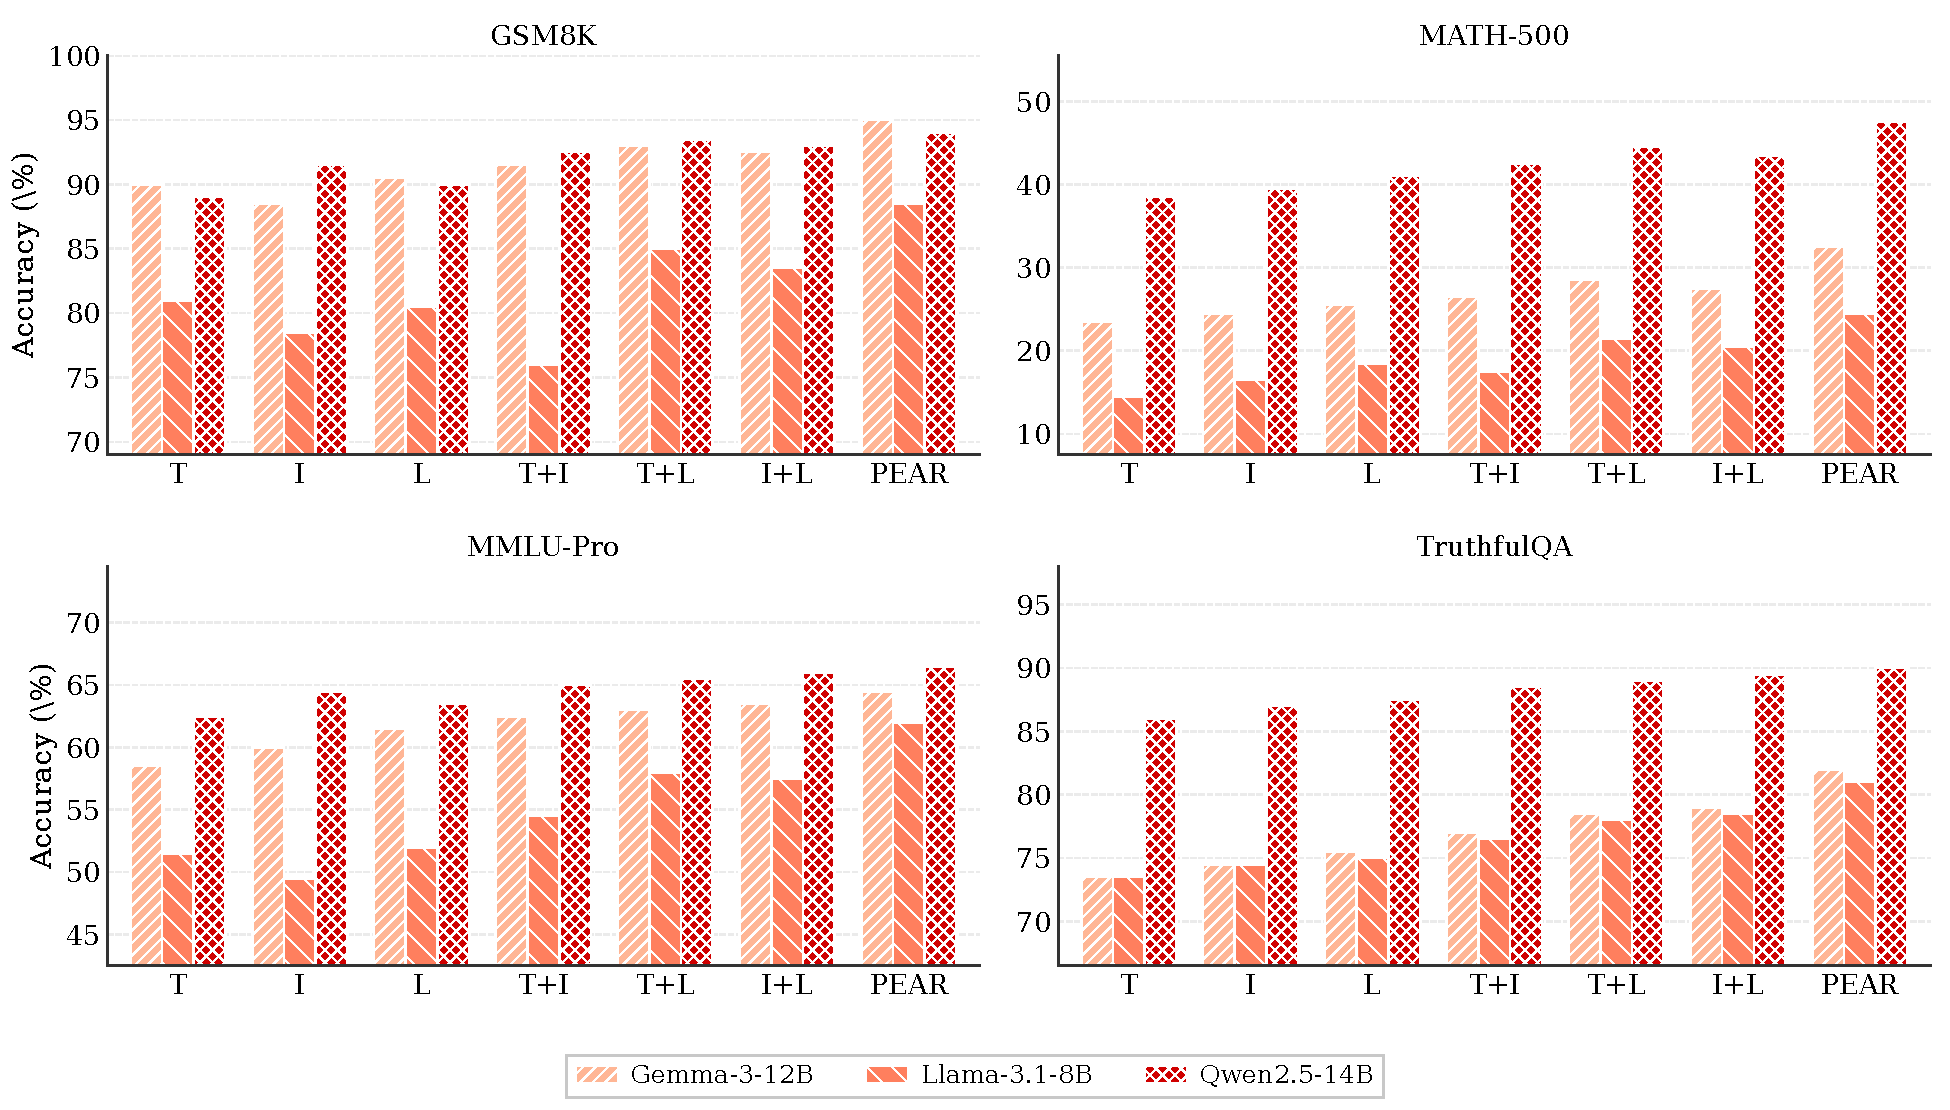
\includegraphics[width=0.95\linewidth]{figs/exps/ablation_bars.pdf}
    \caption{Ablation study of PEAR routing components on open-source models. Targeted = targeted diversity, Influence = influence balancing, LowConf = low-confidence filtering. Each group of bars corresponds to one backbone model; colors indicate routing variant, with PEAR consistently achieving the highest accuracy.}
    \label{fig:ablation}
\end{figure*}



\subsection{Experimental Setup}

\paragraph{Benchmarks.}
We use four benchmarks in knowledge reasoning, factuality, and mathematical reasoning. \textbf{MMLU-Pro}~\cite{wang2024mmlu:mmlu-pro} evaluates broad professional and academic knowledge with multi-step reasoning questions. \textbf{TruthfulQA}~\cite{lin2022truthfulqa:truthfulqa} measures factual reliability and resistance to common misconceptions or false beliefs. \textbf{GSM8K}~\cite{cobbe2021training:gsm8k} focuses on grade-school mathematical word problems that require multi-step arithmetic reasoning. \textbf{MATH-500}~\cite{hendrycks2021measuring:math500} contains competition-level mathematics problems with substantially longer and more complex reasoning chains.

\paragraph{Models.}
We use four open-source instruction-tuned models, namely Gemma-3-12B~\cite{gemmateam2025gemma3technicalreport}, Llama-3.1-8B~\cite{grattafiori2024llama}, Qwen2.5-14B, and Qwen-3-30B-A3B~\cite{yang2025qwen3}, together with two closed-source models, GPT-5.4-nano~\cite{openai2026gpt54} and Claude-Haiku-4.5~\cite{anthropic2025haiku45}. All models are used in the main experiments, while ablation studies are conducted on the three smaller open-source models (Gemma-3-12B, Llama-3.1-8B, and Qwen2.5-14B) to reduce computational cost.


% We compare AR-MAD against the following methods: \textbf{CoT}, a single-agent chain-of-thought baseline; \textbf{CoT-SC}, self-consistency over multiple independent single-agent samples; \textbf{Fixed Clique}, a static fully connected debate graph where each agent observes all others; \textbf{Fixed Star}, a static hub-and-spoke debate graph; \textbf{Fixed Chain}, a static sequential communication graph; \textbf{Fixed Ring}, a static cycle graph where agents communicate with fixed local neighbors; \textbf{Random}, a dynamic sparse baseline where each agent receives critiques from $k$ randomly selected peers per round; and \textbf{AR-MAD}, the complete state-aware routing method combining targeted cross-answer exposure, influence balancing, and low-confidence filtering.
\paragraph{Baselines.}
We compare PEAR against the following baselines: \textbf{CoT}~\cite{wei2022chain:cot}, a single-agent chain-of-thought method; \textbf{CoT-SC}~\cite{wang2022self:sc-cot}, self-consistency over multiple independent samples; and a set of fixed-topology multi-agent debate variants including fully connected (\textbf{Clique}), hub-and-spoke (\textbf{Star}), sequential (\textbf{Chain}), and cyclic (\textbf{Ring}) communication graphs. We further include \textbf{Random}, a dynamic sparse baseline where each agent receives critiques from randomly selected peers at each round.

\paragraph{Metrics.}
We report \textit{round-wise} and \textit{final-answer accuracy} as the main results via majority vote, together with five trajectory-level diagnostics: the wrong-to-right and right-to-wrong update rates (\textit{W2R} / \textit{R2W}), the \textit{critique acceptance rate}, the \textit{cross-answer routing rate} (fraction of routed edges whose source and target hold different answers), \textit{source confidence} (mean source-side confidence in $[0,1]$), and \textit{influence entropy} (normalized entropy of the influence distribution). Detailed definitions are given in Appendix~\ref{app:diagnostics}.


\paragraph{Debate configuration.}
PEAR uses $n=5$ agents and $R=5$ debate rounds. The base topology is $k$-regular with $k=2$, so each target agent receives critiques from two source agents per round.
Further implementation details, including hyperparameter selection, are provided in Appendix~\ref{app:debate}.

\paragraph{Reproducibility.} %More implementation details, p
Prompt templates and a case study of multi-round debate dynamics are in Appendices \ref{app:prompts} and \ref{app:case_study}, respectively. 
The code is available at \url{https://github.com/EVIEHub/PEAR}.
%The code is available at \url{https://anonymous.4open.science/r/PEAR-C8AB/README.md}.



\subsection{Experimental Results}

\paragraph{Overall accuracy.}
% Table~\ref{tab:main-results} reports final-answer accuracy across all model--dataset combinations, spanning four reasoning benchmarks, four open-source backbones, and two closed-source backbones. 
% All open-source models are evaluated on 200 examples per dataset, while closed-source models are evaluated on 100 examples due to API cost constraints. Full-scale results on the complete evaluation sets are reported in Appendix~\ref{app:full-results}.

Table~\ref{tab:main-results} reports final-answer accuracy across all model--dataset combinations. Open-source models are evaluated on 200 examples per dataset and closed-source models on 100 due to API cost constraints; full-scale results are reported in Appendix~\ref{app:full-results}. PEAR achieves the highest accuracy in every row, regardless of dataset, model scale, or provenance. Averaged over all settings, PEAR reaches a mean accuracy of $0.701$, compared with $0.620$ for Fixed Clique, $0.602$ for Fixed Star, $0.610$ for Fixed Chain, and $0.609$ for Fixed Ring. Even when each setting is allowed to pick its single most favorable fixed topology, PEAR still gains $5.1$ points on average.

% AR-MAD achieves the highest accuracy in every row, regardless of dataset, model scale, or open-/closed-source provenance. Averaged over all settings, AR-MAD reaches an overall mean accuracy of $0.701$, compared with $0.620$ for Fixed Clique, $0.602$ for Fixed Star, $0.610$ for Fixed Chain, and $0.609$ for Fixed Ring. Compared with the strongest fixed topology selected \emph{per setting}---a notably tighter baseline than any single static topology---AR-MAD still improves average accuracy by $5.1$ points, indicating that no fixed topology can match the adaptive router even when each setting is allowed to pick its own most favorable static structure.

% Across datasets, AR-MAD improves over the best fixed topology by $6.0$ points on MMLU-Pro, $3.9$ points on TruthfulQA, $4.8$ points on GSM8K, and $5.6$ points on MATH-500. The gains are largest on the two reasoning-heavy benchmarks, MMLU-Pro and MATH-500, where individual agents are more likely to be wrong and therefore benefit most from targeted exposure to dissenting high-confidence sources. The smallest gain occurs on TruthfulQA, where strong models already reach $0.85$--$0.90$ accuracy and the headroom for debate-driven correction is structurally limited; even so, AR-MAD secures the top entry on every row.

% The gains are especially pronounced for weaker backbones: on Llama-3.1-8B, AR-MAD improves over the best fixed topology by $8.0$ points on MMLU-Pro, $9.0$ points on GSM8K, and $9.5$ points on MATH-500. This is consistent with the failure modes diagnosed in Section~\ref{sec:introduction}: when individual agents are weaker, both information homogenization and error cascades have more incorrect material to feed on, so the value of adaptive routing grows. On the strongest open-source backbone, Qwen-3-30B-A3B, AR-MAD's per-row gains shrink to $2.0$--$4.5$ points, but it still wins every row, confirming that the benefit is not confined to weak models.

% Single-agent baselines, including CoT and CoT-SC, lag behind every debate variant across all rows and often by double-digit margins. For example, AR-MAD outperforms CoT by 28.0 points on TruthfulQA with GPT-5.4-nano and by 32.0 points on MATH-500 with Qwen-3-30B-A3B. Self-consistency over independent samples, CoT-SC, closes only a small portion of this gap, indicating that the gains from debate methods arise from inter-agent communication rather than from increasing the number of samples per query.
Per-dataset gains over the best fixed topology are $6.0$ points on MMLU-Pro, $3.9$ on TruthfulQA, $4.8$ on GSM8K, and $5.6$ on MATH-500. The improvement is most pronounced on weaker backbones: on Llama-3.1-8B, PEAR gains $8.0$, $9.0$, and $9.5$ points on MMLU-Pro, GSM8K, and MATH-500 respectively, consistent with the failure modes of fixed-topology debate being more severe when individual agents are weaker. Single-agent baselines such as CoT and CoT-SC trail every debate variant by often double-digit margins, and CoT-SC closes only a small portion of the gap, indicating that the gains arise from inter-agent communication rather than from drawing more samples per query.



\paragraph{Ablation study.}
We ablate the three routing components of PEAR: targeted diversity, influence balancing, and low-confidence filtering. Figure~\ref{fig:ablation} reports accuracy for all single-component, two-component, and full variants on 3 open-source models.
The ablation results show that the full routing objective performs best on average. Among partial variants, combining targeted diversity with low-confidence filtering and combining influence balancing with low-confidence filtering are the strongest, reaching average accuracies of $0.603$ and $0.604$, respectively. The full model reaches $0.657$, suggesting that the three components provide complementary benefits. The improvement is particularly large for Llama-3.1-8B, where PEAR Full substantially outperforms all ablations on GSM8K, MATH-500, MMLU-Pro, and TruthfulQA.

 
\paragraph{Accuracy across debate rounds.}

% To examine how accuracy evolves over the course of a debate, we plot round-wise accuracy for AR-MAD and all baselines on representative open- and closed-source backbones. Figures~\ref{fig:rounds-qwen} and~\ref{fig:rounds-gpt} show the round-by-round trajectories on Qwen-2.5-14B and GPT-5.4-nano, respectively. Across both backbones and all four datasets, AR-MAD consistently achieves higher accuracy at every round and converges to a higher plateau than all fixed-topology baselines. The advantage widens progressively with additional rounds, suggesting that adaptive routing compounds its benefits as the debate proceeds. On Qwen-2.5-14B, AR-MAD improves from $0.284$ at Round~1 to $0.485$ at Round~5 on MATH-500, compared to $0.283$--$0.420$ for the best fixed baseline (Fixed Chain), and from $0.455$ to $0.665$ on MMLU-Pro against $0.453$--$0.620$ for Fixed Chain. On GPT-5.4-nano, the margin is even larger on harder tasks: AR-MAD reaches $0.525$ on MATH-500 by Round~5, surpassing Fixed Clique and Random by $0.070$ points, and achieves $0.730$ on MMLU-Pro against $0.685$ for the next best baseline. On TruthfulQA, where all methods start from a higher base, AR-MAD still maintains a consistent lead, reaching $0.915$ on GPT-5.4-nano compared to $0.845$ for Fixed Clique at Round~5.
%To examine how accuracy evolves over the course of a debate, 
Figures~\ref{fig:rounds-qwen} and~\ref{fig:rounds-gpt} in Appendix~\ref{app:rounds} plot round-wise accuracy on Qwen-2.5-14B and GPT-5.4-nano respectively. Across both backbones and all four datasets, PEAR achieves higher accuracy at every round and converges to a higher plateau than every fixed-topology baseline, with the advantage widening progressively as the debate proceeds. For example, on MATH-500 with Qwen-2.5-14B, PEAR improves from $0.284$ at Round~1 to $0.485$ at Round~5, whereas the strongest fixed baseline saturates at $0.420$. The trend is sharper on harder tasks with GPT-5.4-nano: PEAR reaches $0.525$ on MATH-500 and $0.730$ on MMLU-Pro by Round~5, exceeding the next-best baseline by $0.07$ and $0.045$ points respectively. Even on TruthfulQA, where all methods start from a higher base, PEAR maintains a consistent lead, reaching $0.915$ at Round~5 against $0.845$ for Fixed Clique.



\paragraph{Trajectory-level diagnostics.}
% The diagnostics in Table~\ref{tab:diagnostics} show that AR-MAD improves both correction quality and routing diversity compared to all baselines. It achieves the highest net correction rate of $0.243$, indicating that beneficial updates substantially outweigh harmful flips. More importantly, AR-MAD exhibits substantially higher cross-answer routing at $0.676$, compared to $0.43$--$0.50$ for all baselines, suggesting that the adaptive mechanism effectively encourages information exchange across diverse reasoning trajectories rather than reinforcing local agreement. AR-MAD also yields the highest influence entropy at $0.979$, reflecting a more balanced distribution of influence across agents. Together, these results indicate that performance gains stem from both improved correction dynamics and more diverse communication patterns.
% Detailed metric definitions and additional pattern analyses are provided in Appendix~\ref{app:diagnostics}. 
The diagnostics in Table~\ref{tab:diagnostics} in Appendix~\ref{app:diagnostics} show that PEAR improves both correction quality and routing diversity compared to all baselines. It achieves the highest net correction rate of $0.243$, indicating that beneficial updates substantially outweigh harmful flips, and exhibits substantially higher cross-answer routing at $0.676$ versus $0.43$--$0.50$ for all baselines, suggesting that adaptive routing encourages information exchange across diverse reasoning trajectories rather than reinforcing local agreement. PEAR also yields the highest influence entropy at $0.979$, reflecting a more balanced distribution of influence across agents. Detailed metric definitions and analyses are provided in Appendix~\ref{app:diagnostics}.





\paragraph{Computational overhead.}
% As shown in Figure~\ref{fig:pareto}, AR-MAD lies on the cost--accuracy Pareto frontier on every dataset. We further measure per-example token usage to assess its computational overhead relative to existing debate baselines. AR-MAD consumes about $32.3$k tokens per example, comparable to the Random baseline, which uses the same $k$-regular base graph but selects per-round routing uniformly at random, and $12\%$ lower than the densest Fixed Clique baseline at $36.7$k tokens. Adaptive routing therefore introduces \emph{negligible} additional cost over uniformly random routing under a similar edge budget, while improving average accuracy by $5.7$ points over Random and $6.6$ points over the cheaper Fixed Chain baseline. More details are provided in Appendix~\ref{app:overhead}.
As shown in Figure~\ref{fig:pareto} in Appendix~\ref{app:overhead}, PEAR lies on the cost--accuracy Pareto frontier on every dataset. It consumes about $32.3$k tokens per example, comparable to the Random baseline at the same $k$-regular edge budget and $12\%$ lower than the densest Fixed Clique baseline at $36.7$k tokens. Adaptive routing therefore adds \emph{negligible} cost over uniformly random routing under a similar edge budget, while improving accuracy by $5.7$ points over Random and $6.6$ points over the cheaper Fixed Chain baseline. More details are provided in Appendix~\ref{app:overhead}.




 

 